% =====================================================================
% PEIB (SEES0082) Tutorial 5 - Figure 3 (TikZ, 2 Nov 2026)
% Spec: Claude outputs/Week5/Tutorial/latex/tutorial5_figures_spec.md
%   fig03 semiconductor assembly value chain before and after FDI (schematic)
% Figures 1, 2 and 4 (TikZ pilot) were retired on 2 Nov 2026 to archive.tex: they
% are replaced by the R figures in code/tutorial05_figures.R.
% Build:  py ~/.claude/skills/latex-teaching/scripts/build.py tutorial05_figures.tex --runs 1
% Export: py ~/.claude/skills/latex-teaching/scripts/export_frames.py tutorial05_figures.pdf
%         --out ../../figures/tutorial5 --pages 1 --names tutorial05_fig03_value_chain_fdi
% Page: Beamer with a custom 24 x 12 cm page (\geometry) instead of 4:3; the export
% crops to the ink. The answers toggle below is unused by fig03 (kept for reuse).
% =====================================================================
\documentclass{beamer}
\geometry{paperwidth=24cm,paperheight=12cm}

\usepackage{tikz}
\usepackage{pgfplots}
\usepackage{amsmath}
\usepackage{amssymb}
\usepackage{xcolor}
\usepackage{booktabs}
\usepackage{colortbl}
\usepackage{array}

\usetikzlibrary{decorations.pathreplacing}
\usetikzlibrary{arrows.meta,positioning,patterns}
\pgfplotsset{compat=newest}

\mode<presentation>{
  \usetheme{default}
  \setbeamertemplate{navigation symbols}{}
  \setbeamertemplate{headline}{}
  \setbeamertemplate{footline}{}
}

% PEIB website palette (peib_cols in Teaching_PEIB/code/functions_models.R)
\definecolor{peibdemand}{HTML}{1F3B5C}
\definecolor{peibsupply}{HTML}{8C4A00}
\definecolor{peibcs}{HTML}{4C78A8}
\definecolor{peibps}{HTML}{F58518}
\definecolor{peibtax}{HTML}{54A24B}
\definecolor{peibdwl}{HTML}{E45756}
\definecolor{peibtr}{HTML}{72B7B2}
\definecolor{peibtvc}{HTML}{B279A2}
\definecolor{peibprofit}{HTML}{EECA3B}
\definecolor{peibfc}{HTML}{BAB0AC}

% ANSWERS TOGGLE: 1 = answers variant (PS areas, E1 coordinates), 0 = noanswers variant
\newcommand{\showanswers}{1}

% L-shaped panel axes in economic units, ticks every 10 on both axes
% #1 x max, #2 y max, #3 x-axis label, #4 y-axis label
\newcommand{\panelaxes}[4]{%
  \draw[thick] (0,#2) -- (0,0) -- (#1,0);
  \foreach \t in {0,10,...,#1} {\draw (\t,0) -- ++(0,-2.5pt) node[below, font=\scriptsize] {\t};}
  \foreach \t in {0,10,...,#2} {\draw (0,\t) -- ++(-2.5pt,0) node[left, font=\scriptsize] {\t};}
  \node[below=13pt, font=\footnotesize] at ({#1/2},0) {#3};
  \node[rotate=90, anchor=south, font=\footnotesize] at ([xshift=-17pt]0,{#2/2}) {#4};
}
% rounded integer from an expression (avoids 41.9999 -> 41)
\newcommand{\rint}[2]{\pgfmathtruncatemacro{#1}{round(#2)}}

\tikzset{
  pt/.style={circle, fill=black, inner sep=0pt, minimum size=4pt},
  lab/.style={font=\footnotesize},
  ps/.style={fill=peibps, opacity=0.35},
  guide/.style={dashed, gray},
  curve/.style={very thick},
  shiftarrow/.style={-{Stealth[length=5pt]}, thick, gray},
  leader/.style={gray, thin},
  % same panel size in Figures 1 and 2: 1 unit of Q = 0.11 cm (60 -> 6.6 cm),
  % 1 unit of P = 0.055 cm (120 -> 6.6 cm)
  panel/.style={x=0.11cm, y=0.055cm},
}

\begin{document}

% =====================================================================
% Figure 3: semiconductor assembly value chain before and after FDI (schematic, one variant)
% solid = goods, dashed = payments, dotted = knowledge
% =====================================================================
\begin{frame}[plain,label=fig03]
\centering
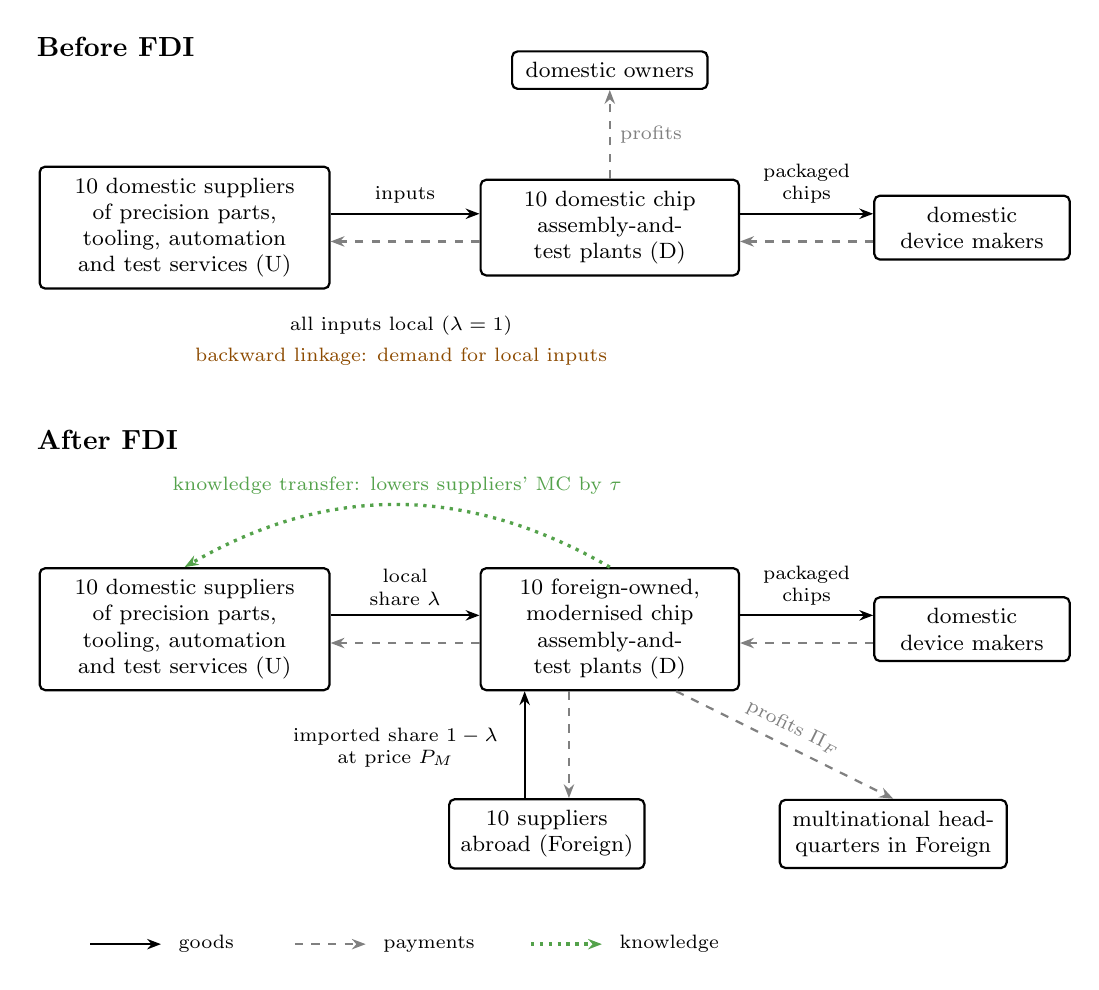
\begin{tikzpicture}[
    box/.style={draw, thick, rounded corners=2pt, align=center, font=\footnotesize, inner sep=4pt},
    goods/.style={-{Stealth[length=5pt]}, thick},
    pay/.style={-{Stealth[length=5pt]}, thick, dashed, gray},
    know/.style={-{Stealth[length=5pt]}, very thick, dotted, peibtax},
    small/.style={font=\scriptsize, align=center},
  ]
  % ---------------- Before FDI ----------------
  \node[font=\bfseries, anchor=west] at (-2.0,2.3) {Before FDI};
  \node[box, text width=3.4cm] (U1) at (0,0) {10 domestic suppliers of precision parts, tooling, automation and test services (U)};
  \node[box, text width=3.0cm] (D1) at (5.4,0) {10 domestic chip assembly-and-test plants (D)};
  \node[box, text width=2.2cm] (M1) at (10.0,0) {domestic device makers};
  \node[box, text width=2.2cm] (O1) at (5.4,2.0) {domestic owners};
  \draw[goods] ([yshift=5pt]U1.east) -- node[above, small] {inputs} ([yshift=5pt]D1.west);
  \draw[pay]   ([yshift=-5pt]D1.west) -- ([yshift=-5pt]U1.east);
  \draw[goods] ([yshift=5pt]D1.east) -- node[above, small] {packaged\\chips} ([yshift=5pt]M1.west);
  \draw[pay]   ([yshift=-5pt]M1.west) -- ([yshift=-5pt]D1.east);
  \draw[pay]   (D1.north) -- node[right, small] {profits} (O1.south);
  \node[small, anchor=north] at (2.75,-1.0) {all inputs local ($\lambda = 1$)};
  \node[small, anchor=north, text=peibsupply] at (2.75,-1.4) {backward linkage: demand for local inputs};

  % ---------------- After FDI ----------------
  \node[font=\bfseries, anchor=west] at (-2.0,-2.7) {After FDI};
  \node[box, text width=3.4cm] (U2) at (0,-5.1) {10 domestic suppliers of precision parts, tooling, automation and test services (U)};
  \node[box, text width=3.0cm] (D2) at (5.4,-5.1) {10 foreign-owned, modernised chip assembly-and-test plants (D)};
  \node[box, text width=2.2cm] (M2) at (10.0,-5.1) {domestic device makers};
  \node[box, text width=2.2cm] (A2) at (4.6,-7.7) {10 suppliers abroad (Foreign)};
  \node[box, text width=2.6cm] (H2) at (9.0,-7.7) {multinational headquarters in Foreign};
  \draw[goods] ([yshift=5pt]U2.east) -- node[above, small] {local\\share $\lambda$} ([yshift=5pt]D2.west);
  \draw[pay]   ([yshift=-5pt]D2.west) -- ([yshift=-5pt]U2.east);
  \draw[goods] ([yshift=5pt]D2.east) -- node[above, small] {packaged\\chips} ([yshift=5pt]M2.west);
  \draw[pay]   ([yshift=-5pt]M2.west) -- ([yshift=-5pt]D2.east);
  \draw[goods] ([xshift=-8pt]A2.north) -- ([xshift=-8pt]A2.north |- D2.south);
  \draw[pay]   ([xshift=8pt]A2.north |- D2.south) -- ([xshift=8pt]A2.north);
  \node[small, anchor=east] at (4.1,-6.6) {imported share $1 - \lambda$\\at price $P_M$};
  \draw[pay]   ([xshift=24pt]D2.south) -- node[sloped, above, small] {profits $\Pi_F$} (H2.north);
  \draw[know]  (D2.north) to[out=150, in=30] node[above, small, text=peibtax] {knowledge transfer: lowers suppliers' MC by $\tau$} (U2.north);

  % ---------------- legend ----------------
  \begin{scope}[shift={(-1.2,-9.1)}]
    \draw[goods] (0,0) -- (0.9,0); \node[small, anchor=west] at (1.0,0) {goods};
    \draw[pay]   (2.6,0) -- (3.5,0); \node[small, anchor=west] at (3.6,0) {payments};
    \draw[know]  (5.6,0) -- (6.5,0); \node[small, anchor=west] at (6.6,0) {knowledge};
  \end{scope}
\end{tikzpicture}
\end{frame}


\end{document}
